\section{Marco teórico específico}

El \emph{Common Gateway Interface} (CGI) es la primera especificación que permitió a un servidor web ejecutar un programa externo para generar dinámicamente la respuesta a una petición HTTP. Desde la perspectiva de la arquitectura RPC, cada invocación HTTP a un script CGI equivale a una llamada a un procedimiento remoto cuyo formato de entrada son las variables de entorno estándar (\texttt{REQUEST\_METHOD}, \texttt{QUERY\_STRING}, \texttt{CONTENT\_LENGTH}, \texttt{HTTP\_ACCEPT}, \texttt{REMOTE\_ADDR}, entre otras) y cuyo formato de salida son los encabezados HTTP seguidos de una línea en blanco y el cuerpo de la respuesta, escrito en \texttt{stdout} del proceso~\cite{techtarget2024rpc}.

A diferencia de Apache HTTP Server, que ejecuta CGI de forma nativa mediante el módulo \texttt{mod\_cgi}, nginx no incluye soporte directo para CGI: por diseño solo entiende los protocolos FastCGI, uWSGI y SCGI, ya que su modelo de ejecución es asíncrono y dirigido por eventos, en contraste con el modelo de Apache basado en procesos o hilos, que puede permitirse bloquear un \emph{worker} mientras hace \texttt{fork}/\texttt{exec} de un script. Por esta razón se utiliza \texttt{fcgiwrap}, un demonio que actúa como adaptador: escucha peticiones FastCGI en un socket Unix (\texttt{/run/fcgiwrap.socket}) y, por cada una, lanza el script CGI clásico como proceso hijo, alimentándolo con las variables de entorno y el \texttt{stdin}/\texttt{stdout} que la convención CGI espera~\cite{f5nginx2023fcgiwrap,ubuntu2023fcgiwrap}.

\section{Entorno de trabajo}

Siguiendo lo descrito en la Sección de entorno común (véase Tabla~\ref{tab:entorno-comun}), esta práctica se desarrolló en un contenedor Docker con imagen \texttt{fedora:36}, publicando el puerto 80 del contenedor en el puerto 8080 del anfitrión.

\begin{figure}[H]
\centering
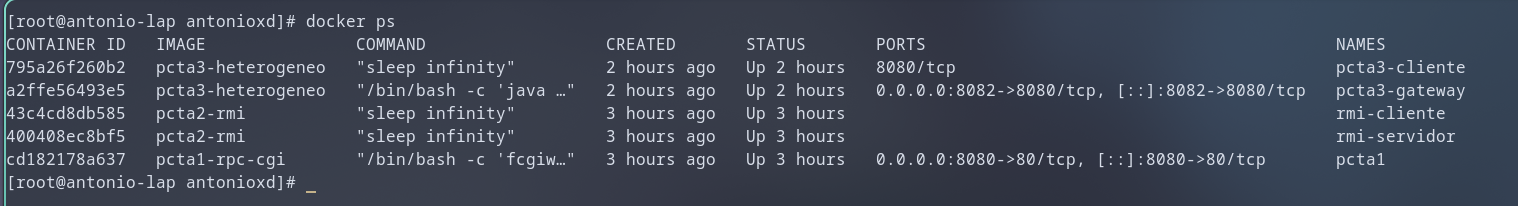
\includegraphics[width=\linewidth]{../src/ss/2.1.png}
\caption{Contenedor \texttt{pcta1} en ejecución con el mapeo de puertos \texttt{8080$\rightarrow$80}.}
\label{fig:p1-docker-ps}
\end{figure}

En la Figura~\ref{fig:p1-docker-ps} se observa el contenedor \texttt{pcta1} (imagen \texttt{pcta1-rpc-cgi}) con el mapeo \texttt{0.0.0.0:8080->80/tcp}: Docker inserta una regla de traducción de direcciones (NAT) que reenvía el tráfico del puerto 8080 del anfitrión al puerto 80 interno donde escucha nginx. Desde la perspectiva del modelo RPC, este mapeo forma parte del \emph{runtime}: es infraestructura de transporte que el cliente no necesita conocer —invoca \texttt{localhost:8080} como si el servidor fuera local, primera manifestación de la transparencia que persigue el modelo~\cite{birrell1984rpc}. La columna \texttt{COMMAND} muestra además el arranque conjunto de \texttt{fcgiwrap} y nginx, los dos procesos que constituyen el lado servidor del \emph{runtime}.

\section{Instalación de nginx y fcgiwrap}

Se instalaron los paquetes equivalentes a los solicitados en el instructivo (\texttt{apt install nginx fcgiwrap curl jq} $\rightarrow$ \texttt{dnf install nginx fcgiwrap curl jq bc} en Fedora):

\begin{lstlisting}[language=bash]
RUN dnf install -y nginx fcgiwrap bc curl jq procps-ng && dnf clean all
\end{lstlisting}

\begin{figure}[H]
\centering
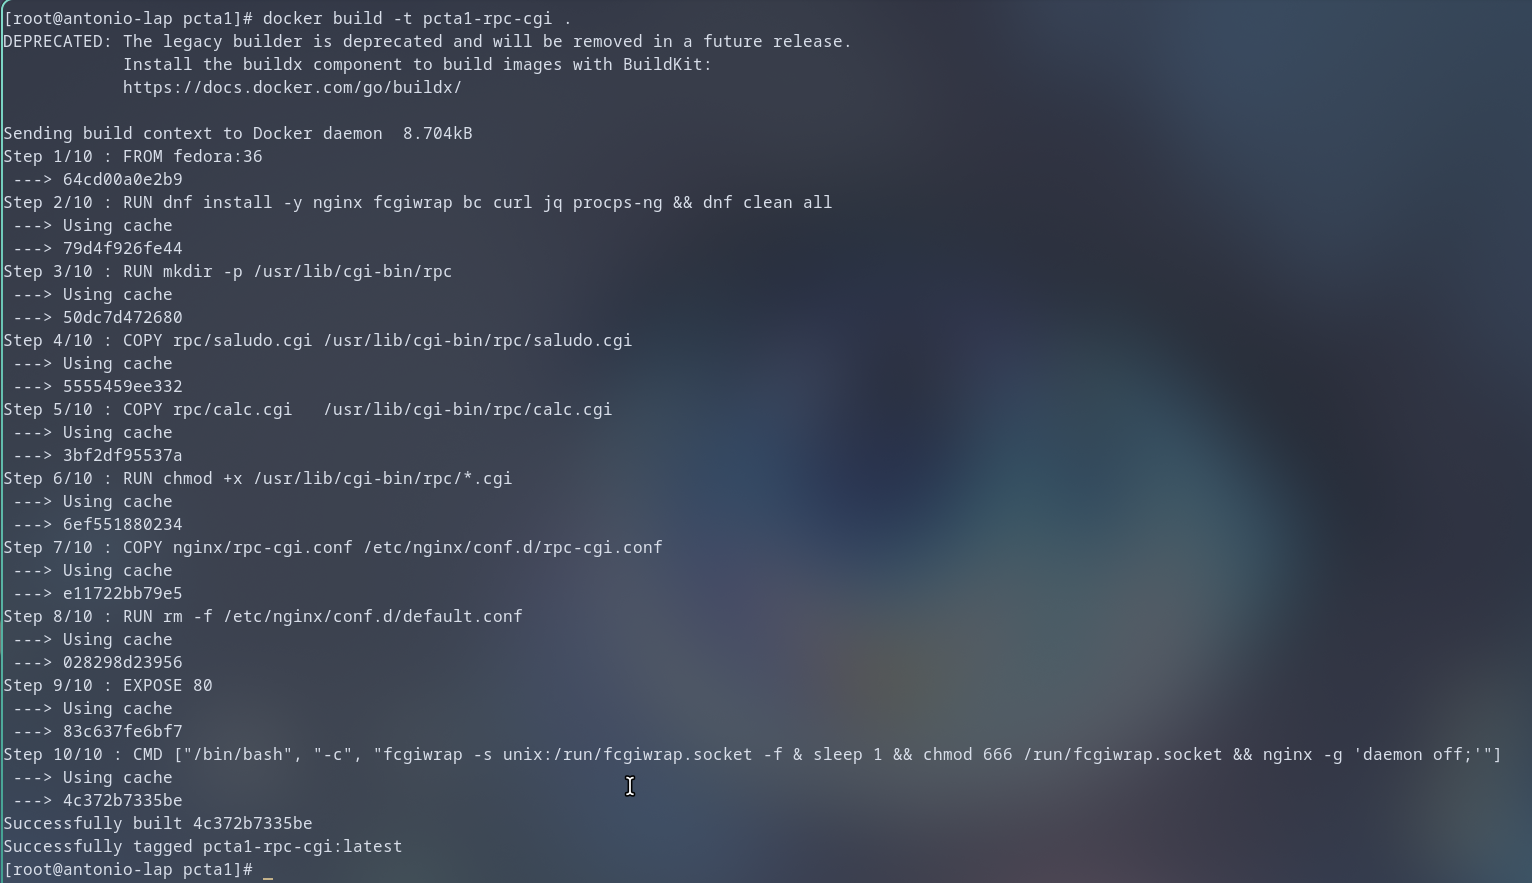
\includegraphics[width=\linewidth]{../src/ss/2.2.png}
\caption{Construcción de la imagen \texttt{pcta1-rpc-cgi}: instalación de paquetes, despliegue de los scripts CGI y configuración de nginx.}
\label{fig:p1-install}
\end{figure}

La Figura~\ref{fig:p1-install} muestra los diez pasos de construcción de la imagen. Cada instrucción del \texttt{Dockerfile} produce una capa inmutable identificada por un \emph{hash} (las líneas \texttt{Using cache} indican que la capa ya existía de una construcción previa y se reutiliza sin re-ejecutar el paso, lo que hace la construcción reproducible e incremental). Los pasos relevantes para el modelo RPC son: la instalación de nginx y \texttt{fcgiwrap} (paso 2, el \emph{runtime}), la copia de \texttt{saludo.cgi} y \texttt{calc.cgi} al directorio estándar \texttt{/usr/lib/cgi-bin/rpc} (pasos 4--5, el servidor), el bit de ejecución sobre los scripts (paso 6, requisito para que \texttt{fcgiwrap} pueda hacer \texttt{exec} de ellos) y la configuración del \emph{location} de nginx (paso 7, la tabla de ruteo que asocia la URL pública con el procedimiento).

\section{Script CGI bash: procedimiento remoto \texttt{saludo}}

Se implementó \texttt{/usr/lib/cgi-bin/rpc/saludo.cgi} conforme al instructivo: lee el parámetro \texttt{nombre} desde \texttt{QUERY\_STRING} (GET) o desde el cuerpo (POST), decodifica el valor y responde en texto plano o JSON según la cabecera \texttt{Accept}.

\section{Configuración de nginx}

Se configuró \texttt{/etc/nginx/conf.d/rpc-cgi.conf} enrutando \texttt{/rpc/} hacia el socket de \texttt{fcgiwrap}:

\begin{lstlisting}
location /rpc/ {
    gzip off;
    root /usr/lib/cgi-bin;
    fastcgi_pass unix:/run/fcgiwrap.socket;
    fastcgi_index index.cgi;
    include /etc/nginx/fastcgi_params;
    fastcgi_param SCRIPT_FILENAME $document_root$fastcgi_script_name;
    fastcgi_param DOCUMENT_ROOT   $document_root;
}
\end{lstlisting}

\section{Invocación remota desde el cliente}

\subsection*{Invocación tipo GET}
\begin{lstlisting}[language=bash]
$ curl -s 'http://localhost:8080/rpc/saludo.cgi?nombre=Antonio'
Hola, Antonio -- petición desde 172.17.0.1
\end{lstlisting}

\begin{figure}[H]
\centering
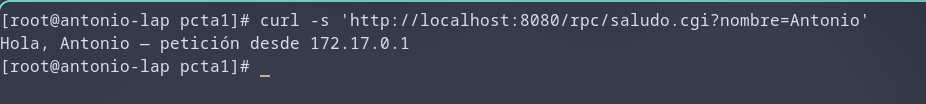
\includegraphics[width=\linewidth]{../src/ss/2.3.png}
\caption{Invocación remota por método GET: el parámetro viaja en la URL.}
\label{fig:p1-get}
\end{figure}

En la Figura~\ref{fig:p1-get}, el parámetro \texttt{nombre=Antonio} viaja como parte de la URL (\emph{query string}). Del lado servidor, nginx coloca esa cadena en la variable de entorno \texttt{QUERY\_STRING} —tal como exige la especificación CGI— y el script la extrae con \texttt{sed}. Este trayecto es exactamente el \emph{marshalling}/\emph{unmarshalling} de la arquitectura clásica: el cliente (curl) serializa el argumento en un formato de transporte (URL codificada) y el stub del servidor (las primeras líneas del script) lo deserializa a una variable local de bash. La respuesta incluye \texttt{172.17.0.1}, valor de \texttt{REMOTE\_ADDR}: la dirección de la puerta de enlace del \emph{bridge} de Docker, que demuestra que la petición efectivamente atravesó una frontera de red y no fue una llamada local.

\subsection*{Invocación tipo POST}
\begin{lstlisting}[language=bash]
$ curl -s -X POST -d 'nombre=ESIME' http://localhost:8080/rpc/saludo.cgi
Hola, ESIME -- petición desde 172.17.0.1
\end{lstlisting}

\begin{figure}[H]
\centering
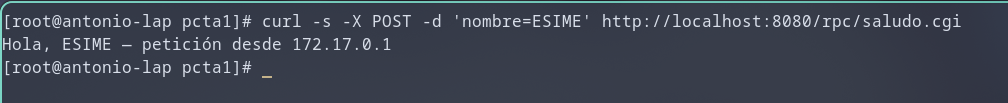
\includegraphics[width=\linewidth]{../src/ss/2.4.png}
\caption{Invocación remota por método POST: el parámetro viaja en el cuerpo de la petición.}
\label{fig:p1-post}
\end{figure}

La Figura~\ref{fig:p1-post} repite la invocación con el método POST: el mismo parámetro ya no viaja en la URL sino en el cuerpo de la petición HTTP. El contrato CGI cambia en consecuencia: nginx anuncia la longitud del cuerpo en \texttt{CONTENT\_LENGTH} y lo entrega por la \emph{entrada estándar} del script, que lo lee con \texttt{head -c "\$CONTENT\_LENGTH"}. Que el mismo procedimiento acepte ambos métodos ilustra que en RPC el formato de serialización de los argumentos es un detalle del protocolo de transporte, negociable sin cambiar la semántica del procedimiento: el resultado observable es idéntico en ambos casos.

\subsection*{Solicitud con representación JSON}
\begin{lstlisting}[language=bash]
$ curl -s -H 'Accept: application/json' \
    'http://localhost:8080/rpc/saludo.cgi?nombre=Profesor' | jq .
{
  "servicio": "saludo",
  "resultado": "Hola, Profesor",
  "origen": "172.17.0.1"
}
\end{lstlisting}

\begin{figure}[H]
\centering
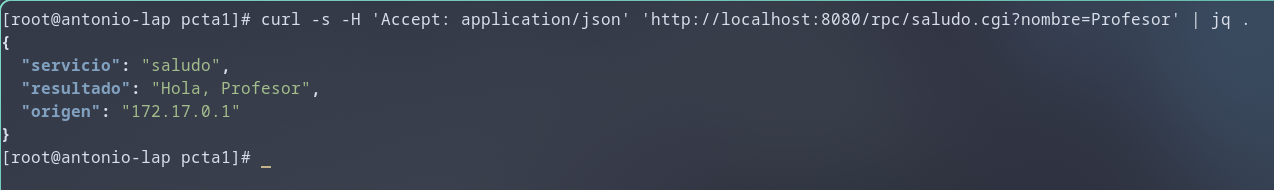
\includegraphics[width=\linewidth]{../src/ss/2.5.png}
\caption{Negociación de contenido: la cabecera \texttt{Accept: application/json} selecciona la representación JSON de la respuesta.}
\label{fig:p1-json}
\end{figure}

En la Figura~\ref{fig:p1-json} el cliente añade la cabecera \texttt{Accept: application/json}, que nginx traslada al script como la variable \texttt{HTTP\_ACCEPT}; el script la inspecciona y elige la rama que serializa la respuesta como JSON en lugar de texto plano. Este mecanismo —negociación de contenido— realiza la tercera propiedad de un sistema RPC bien diseñado enunciada en el marco teórico: la \emph{independencia de la representación de datos}. El procedimiento es el mismo y el argumento es el mismo; solo cambia el formato acordado entre las partes para el resultado, sin modificar ni al cliente ni a la lógica del servidor.

\subsection*{Verificación de códigos de estado HTTP}
\begin{lstlisting}[language=bash]
$ curl -sD - -o /dev/null 'http://localhost:8080/rpc/saludo.cgi?nombre=Mike'
HTTP/1.1 200 OK

$ curl -sD - -o /dev/null -X PUT 'http://localhost:8080/rpc/saludo.cgi?nombre=x'
HTTP/1.1 405 Method Not Allowed
\end{lstlisting}

Las invocaciones anteriores reproducen el comportamiento descrito en el instructivo: la dirección de origen (\texttt{172.17.0.1}) corresponde a la puerta de enlace del \emph{bridge} de Docker, análoga a la \texttt{127.0.0.1} que se obtendría al invocar desde la misma máquina en un entorno sin contenedores.

\section{Identificación de los cinco componentes RPC}

\begin{table}[H]
\centering
\caption{Asociación de la práctica 1 con la arquitectura clásica de RPC.}
\label{tab:componentes-rpc-p1}
\begin{tabularx}{\linewidth}{lX}
\toprule
\textbf{Componente RPC} & \textbf{Realización en la práctica 1} \\
\midrule
Cliente & \texttt{curl} invocando una URL con parámetros. \\
Stub del cliente & \texttt{libcurl}: arma la línea de petición HTTP, codifica \texttt{QUERY\_STRING} o el cuerpo y serializa los encabezados. \\
RPC runtime & \texttt{nginx} + \texttt{fcgiwrap}: gestionan TCP, el protocolo FastCGI, el mapeo de variables y la devolución de la respuesta. \\
Stub del servidor & La lógica de \texttt{saludo.cgi} que parsea las variables de entorno CGI hacia la variable bash \texttt{nombre}. \\
Servidor & El cuerpo del script (rama \texttt{if}/\texttt{else}) que produce el mensaje y lo emite por \texttt{stdout}. \\
\bottomrule
\end{tabularx}
\end{table}

\begin{figure}[H]
\centering

\includegraphics[width=0.9\linewidth]{../src/diagrams/practica1_secuencia.png}
\caption{Diagrama de secuencia de la invocación remota en la práctica 1.}
\label{fig:p1-secuencia}
\end{figure}
